\documentclass[onlymath]{beamer}
% \documentclass[onlymath,handout]{beamer}

% Macros used by all lectures, but not necessarily by excercises

%%% General setup and dependencies:

% \usetheme[ddcfooter,nosectionnum]{tud}
\usetheme[nosectionnum,pagenum,noheader]{tud}
% \usetheme[nosectionnum,pagenum]{tud}

% Increase body font size to a sane level:
\let\origframetitle\frametitle
% \renewcommand{\frametitle}[1]{\origframetitle{#1}\normalsize}
\renewcommand{\frametitle}[1]{\origframetitle{#1}\fontsize{10pt}{13.2}\selectfont}
\setbeamerfont{itemize/enumerate subbody}{size=\small} % tud defaults to scriptsize!
\setbeamerfont{itemize/enumerate subsubbody}{size=\small}
% \setbeamerfont{normal text}{size=\small}
% \setbeamerfont{itemize body}{size=\small}

\renewcommand{\emph}[1]{\textbf{#1}}

\def\arraystretch{1.3}% Make tables even less cramped vertically

\usepackage[ngerman]{babel}
\usepackage[utf8]{inputenc}
\usepackage[T1]{fontenc}

%\usepackage{graphicx}
\usepackage[export]{adjustbox} % loads graphicx
\usepackage{import}
\usepackage{stmaryrd}
\usepackage[normalem]{ulem} % sout command
% \usepackage{times}
\usepackage{txfonts}
\usepackage{array}

% \usepackage[perpage]{footmisc} % reset footnote counter on each page -- fails with beamer (footnotes gone)
\usepackage{perpage}  % reset footnote counter on each page
\MakePerPage{footnote}

\usepackage{tikz}
\usetikzlibrary{arrows,positioning,decorations.pathreplacing}
% Inspired by http://www.texample.net/tikz/examples/hand-drawn-lines/
\usetikzlibrary{decorations.pathmorphing}
\pgfdeclaredecoration{penciline}{initial}{
    \state{initial}[width=+\pgfdecoratedinputsegmentremainingdistance,
    auto corner on length=1mm,]{
        \pgfpathcurveto%
        {% From
            \pgfqpoint{\pgfdecoratedinputsegmentremainingdistance}
                      {\pgfdecorationsegmentamplitude}
        }
        {%  Control 1
        \pgfmathrand
        \pgfpointadd{\pgfqpoint{\pgfdecoratedinputsegmentremainingdistance}{0pt}}
                    {\pgfqpoint{-\pgfdecorationsegmentaspect
                     \pgfdecoratedinputsegmentremainingdistance}%
                               {\pgfmathresult\pgfdecorationsegmentamplitude}
                    }
        }
        {%TO
        \pgfpointadd{\pgfpointdecoratedinputsegmentlast}{\pgfpoint{1pt}{1pt}}
        }
    }
    \state{final}{}
}
\tikzset{handdrawn/.style={decorate,decoration=penciline}}
\tikzset{every shadow/.style={fill=none,shadow xshift=0pt,shadow yshift=0pt}}
% \tikzset{module/.append style={top color=\col,bottom color=\col}}

% Use to make Tikz attributes with Beamer overlays
% http://tex.stackexchange.com/a/6155
\tikzset{onslide/.code args={<#1>#2}{%
  \only<#1| handout:0>{\pgfkeysalso{#2}}
}}
\tikzset{onslideprint/.code args={<#1>#2}{%
  \only<#1>{\pgfkeysalso{#2}}
}}

%%% Title -- always set this first

\newcommand{\defineTitle}[3]{
	\newcommand{\lectureindex}{#1}
	\title{Theoretische Informatik und Logik}
	\subtitle{\href{\lectureurl}{#1. Vorlesung: #2}}
	\author{\href{https://iccl.inf.tu-dresden.de/web/Markus_Kr\%C3\%B6tzsch}{Markus Kr\"{o}tzsch}\\[1ex]Lehrstuhl Wissensbasierte Systeme}
	\date{#3}
	\datecity{TU Dresden}
% 	\institute{CC-By 3.0, sofern keine anderslautenden Bildrechte angegeben sind}
}

%%% Table of contents:

\RequirePackage{ifthen}

\newcommand{\highlight}[2]{%
	\ifthenelse{\equal{#1}{\lectureindex}}{\alert{#2}}{#2}%
}

\def\myspace{-0.7ex}
\newcommand{\printtoc}{
\begin{tabular}{r@{$\quad$}l}
\highlight{1}{1.} & \highlight{1}{Willkommen/Einleitung formale Sprachen}\\[\myspace]
\highlight{2}{2.} & \highlight{2}{Grammatiken und die Chomsky-Hierarchie}\\[\myspace]
\highlight{3}{3.} & \highlight{3}{Endliche Automaten}\\[\myspace]
\highlight{4}{4.} & \highlight{4}{Complexity of FO query answering}\\[\myspace]
\highlight{5}{5.} & \highlight{5}{Conjunctive queries}\\[\myspace]
\highlight{6}{6.} & \highlight{6}{Tree-like conjunctive queries}\\[\myspace]
\highlight{7}{7.} & \highlight{7}{Query optimisation}\\[\myspace]
\highlight{8}{8.} & \highlight{8}{Conjunctive Query Optimisation / First-Order~Expressiveness}\\[\myspace]
\highlight{9}{9.} & \highlight{9}{First-Order~Expressiveness / Introduction to Datalog}\\[\myspace]
\highlight{10}{10.} & \highlight{10}{Expressive Power and Complexity of Datalog}\\[\myspace]
\highlight{11}{11.} & \highlight{11}{Optimisation and Evaluation of Datalog}\\[\myspace]
\highlight{12}{12.} & \highlight{12}{Evaluation of Datalog (2)}\\[\myspace]
\highlight{13}{13.} & \highlight{13}{Graph Databases and Path Queries}\\[\myspace]
\highlight{14}{14.} & \highlight{14}{Outlook: database theory in practice}
\end{tabular}
}

\newcommand{\overviewslide}{%
\begin{frame}\frametitle{Overview}
\printtoc
\medskip

Siehe \href{\lectureurl}{course homepage [$\Rightarrow$ link]} for more information and materials
\end{frame}
}

%%% Colours:
\usepackage{xcolor,colortbl}
\definecolor{redhighlights}{HTML}{FFAA66}
\definecolor{lightblue}{HTML}{55AAFF}
\definecolor{lightred}{HTML}{FF5522}
\definecolor{lightpurple}{HTML}{DD77BB}
\definecolor{lightgreen}{HTML}{55FF55}
\definecolor{darkred}{HTML}{CC4411}
\definecolor{darkblue}{HTML}{176FC0}%{1133AA}
\definecolor{nightblue}{HTML}{2010A0}%{1133AA}
\definecolor{alert}{HTML}{176FC0}
\definecolor{darkgreen}{HTML}{36AB14}
\definecolor{strongyellow}{HTML}{FFE219}
\definecolor{devilscss}{HTML}{666666}

\newcommand{\redalert}[1]{\textcolor{darkred}{#1}}

%%% Slide layout commands:

\newcommand{\sectionSlide}[1]{
\frame{\begin{center}
\LARGE
#1
\end{center}}
}
\newcommand{\sectionSlideNoHandout}[1]{
\frame<handout:0>{\begin{center}
\LARGE
#1
\end{center}}
}

\newcommand{\mydualbox}[3]{%
 \begin{minipage}[t]{#1}
 \begin{beamerboxesrounded}[upper=block title,lower=block body,shadow=true]%
    {\centering\usebeamerfont*{block title}#2}%
    \raggedright%
    \usebeamerfont{block body}
%     \small
    #3%
  \end{beamerboxesrounded}
  \end{minipage}
}
%
\newcommand{\myheaderbox}[2]{%
 \begin{minipage}[t]{#1}
 \begin{beamerboxesrounded}[upper=block title,lower=block title,shadow=true]%
    {\centering\usebeamerfont*{block title}\rule{0pt}{2.6ex} #2}%
  \end{beamerboxesrounded}
  \end{minipage}
}

\newcommand{\mycontentbox}[2]{%
 \begin{minipage}[t]{#1}%
 \begin{beamerboxesrounded}[upper=block body,lower=block body,shadow=true]%
    {\centering\usebeamerfont*{block body}\rule{0pt}{2.6ex}#2}%
  \end{beamerboxesrounded}
  \end{minipage}
}

\newcommand{\mylcontentbox}[2]{%
 \begin{minipage}[t]{#1}%
 \begin{beamerboxesrounded}[upper=block body,lower=block body,shadow=true]%
    {\flushleft\usebeamerfont*{block body}\rule{0pt}{2.6ex}#2}%
  \end{beamerboxesrounded}
  \end{minipage}
}

% label=180:{\rotatebox{90}{{\footnotesize\textcolor{darkgreen}{Beispiel}}}}
% \hspace{-8mm}\ghost{\raisebox{-7mm}{\rotatebox{90}{{\footnotesize\textcolor{darkgreen}{Beispiel}}}}}\hspace{8mm}
\newcommand{\examplebox}[1]{%
	\begin{tikzpicture}[decoration=penciline, decorate]
		\pgfmathsetseed{1235}
		\node (n1) [decorate,draw=darkgreen, fill=darkgreen!10,thick,align=left,text width=\linewidth, inner ysep=2mm, inner xsep=2mm] at (0,0) {#1};
% 		\node (n2) [align=left,text width=\linewidth,inner sep=0mm] at (n1.92) {{\footnotesize\raisebox{3mm}{\textcolor{darkgreen}{Beispiel}}}};
% 		\node (n2) [decorate,draw=darkgreen, fill=darkgreen!10,thick, align=left,text width=\linewidth,inner sep=2mm] at (n1.90) {{\footnotesize\raisebox{0mm}{\textcolor{darkgreen}{Beispiel}}}};
	\end{tikzpicture}%
}%

\newcommand{\codebox}[1]{%
	\begin{tikzpicture}[decoration=penciline, decorate]
		\pgfmathsetseed{1236}
		\node (n1) [decorate,draw=strongyellow, fill=strongyellow!10,thick,align=left,text width=\linewidth, inner ysep=2mm, inner xsep=2mm] at (0,0) {#1};
	\end{tikzpicture}%
}%

\newcommand{\defbox}[1]{%
	\begin{tikzpicture}[decoration=penciline, decorate]
		\pgfmathsetseed{1237}
		\node (n1) [decorate,draw=darkred, fill=darkred!10,thick,align=left,text width=\linewidth, inner ysep=2mm, inner xsep=2mm] at (0,0) {#1};
	\end{tikzpicture}%
}%

\newcommand{\theobox}[1]{%
	\begin{tikzpicture}[decoration=penciline, decorate]
		\pgfmathsetseed{1240}
		\node (n1) [decorate,draw=darkblue, fill=darkblue!10,thick,align=left,text width=\linewidth, inner ysep=2mm, inner xsep=2mm] at (0,0) {#1};
	\end{tikzpicture}%
}%

\newcommand{\anybox}[2]{%
	\begin{tikzpicture}[decoration=penciline, decorate]
		\pgfmathsetseed{1240}
		\node (n1) [decorate,draw=#1, fill=#1!10,thick,align=left,text width=\linewidth, inner ysep=2mm, inner xsep=2mm] at (0,0) {#2};
	\end{tikzpicture}%
}%


\newsavebox{\mybox}%
\newcommand{\doodlebox}[2]{%
\sbox{\mybox}{#2}%
	\begin{tikzpicture}[decoration=penciline, decorate]
		\pgfmathsetseed{1238}
		\node (n1) [decorate,draw=#1, fill=#1!10,thick,align=left,inner sep=1mm] at (0,0) {\usebox{\mybox}};
	\end{tikzpicture}%
}%


\defineTitle{9}{NP und NP-Vollständigkeit}{10. Mai 2017}

\begin{document}

\maketitle

\begin{frame}\frametitle{Rückblick}

\Scomplclass{PTime} und \Scomplclass{LogSpace} als mathematische Modelle für Effizienz:
\begin{itemize}
\item \Scomplclass{PTime} als robuste Verallgemeinerung der in linearer Zeit lösbaren Probleme
\item \Scomplclass{LogSpace} als typische (vermutlich) subpolynomielle Klasse
\end{itemize}\bigskip

\emph{Wichtige Anwendung:} Reduktionen, die ein Problem mit wenig Aufwand auf ein anderes zurückführen
\begin{itemize}
\item \alert{Polynomielle (Many-One-)Reduktionen:} verbreitetste Form von effizienter Reduktion; Notation: $\leq_p$
\item \alert{\Scomplclass{LogSpace}-Reduktionen:} häufig anzutreffen, aber selten im Detail definiert
\end{itemize}

\end{frame}

\begin{frame}\frametitle{Warum sollten Reduktionen effizient sein?}

\emph{Intuition:} Eine aufwändige Reduktion kann jedes Problem indirekt lösen, aber dadurch lernt man nichts
interessantes über dessen Komplexität.\pause
\bigskip

\theobox{Satz: Sei $\Slang{L}=\{\Sterm{a}\}$ eine Sprache über dem Alphabet $\{\Sterm{a}\}$.
Falls $\Slang{P}$ entscheidbar ist, dann gibt es eine Many-One-Reduktion $\Slang{P}\leq_m\Slang{L}$.}\pause

\emph{Beweis:} Die Reduktion $f$ funktioniert wie folgt:
\begin{itemize}
\item Wenn $w\in \Slang{P}$, dann sei $f(w)=\Sterm{a}$.
\item Andernfalls, wenn $w\notin \Slang{P}$, dann sei $f(w)=\Sterm{aa}$.\qed
\end{itemize}

\end{frame}


\begin{frame}\frametitle{Effizient und doch nicht praktikabel}

Es gibt Situationen, in denen ein Problem in \Scomplclass{PTime} liegt 
und dennoch nicht praktisch algorithmisierbar ist.\medskip

\theobox{Satz: Jede endliche Sprache kann in $\Scomplclass{DTIME}(1)$ erkannt werden und liegt daher
insbesondere in \Scomplclass{PTime} und \Scomplclass{LogSpace}.}\bigskip\pause

\examplebox{Beispiel: Sei $\Slang{L}$ die Sprache, die alle wahren Aussagen aus der
folgenden Menge enthält: $\{"`\Scomplclass{P}=\Scomplclass{NP}"', "`\Scomplclass{P}\neq\Scomplclass{NP}"'\}$. Dann ist $\Slang{L}\in\Scomplclass{PTime}$ und damit effizient berechenbar.}\pause

\emph{Erkenntnis:} Man kann manchmal die Existenz eines effizienten Algorithmus beweisen,
ohne zu wissen, wie er aussehen müsste.\\
$\leadsto$ \alert{nichtkonstruktiver Beweis}


\end{frame}

\sectionSlide{\Scomplclass{NP}}

\begin{frame}\frametitle{Der Vortrag ohne Worte}

~\hfill
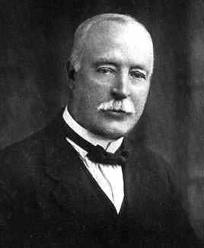
\includegraphics[height=5cm]{images/Cole}
\hfill~

~\hfill
Frank Nelson Cole
\hfill~

\end{frame}


\begin{frame}\frametitle{Rückblick: Polynomielle Verifikatoren}

In der Vorlesung Formale Systeme haben wir die folgende Definition kennengelernt:

\defbox{Ein \redalert{polynomieller Verifikator} für eine Sprache $\Slang{L}\subseteq \Sigma^*$ ist eine
polynomiell-zeitbeschränkte, deterministische TM \Smach{M}, für die gilt:
\begin{itemize}
\item \Smach{M} akzeptiert nur Wörter der Form $w\# z$ mit:
	\begin{itemize}
	\item $w\in\Slang{L}$
	\item $z\in\Sigma^*$ ist ein \redalert{Zertifikat} polynomieller Länge\\(d.h. für \Smach{M} gibt es ein Polynom $p$ mit $|z|\leq p(|w|)$)
	\end{itemize}
\item Für jedes Wort $w\in\Slang{L}$ gibt es ein solches Wort $w\# z\in\Slang{L}(\Smach{M})$.
\end{itemize}
}

\emph{Intuition:}
\begin{itemize}
\item Das Zertifikat $z$ kodiert die Lösung des Problems $w$, die der Verifikator lediglich nachprüft.
\item Zertifikate sollten kurz sein, damit die Prüfung selbst nicht länger dauert als die Lösung des Problems.
\end{itemize}

Zertifikate werden auch \alert{Nachweis}, \alert{Beweis} oder \alert{Zeuge} genannt

\end{frame}

\begin{frame}\frametitle{Rückblick: Nachweis-polynomielle Sprachen}

% Wir haben \Scomplclass{NP} definiert als $\Scomplclass{NP} = \bigcup_{k\geq 1} \Scomplclass{NTime}(n^k)$.
% \bigskip

Daraus ergibt sich die Definition einer Sprachklasse:

\defbox{Eine Sprache $\Slang{L}$ ist \redalert{nachweis-polynomiell} wenn es für sie einen polynomiellen
Verifikator gibt.}\medskip\pause

\examplebox{Beispiel: Die Entscheidung, ob ein gegebener Graph einen Hamilton-Pfad zulässt, ist nachweis-polynomiell.
Als Zertifikat dient der entsprechende Pfad.}\bigskip

\end{frame}

\begin{frame}\frametitle{\Scomplclass{NP} bedeutet "`nachweis-polynomiell"'}

Wir hatten sodann gezeigt:\medskip

\theobox{Satz: Eine Sprache $\Slang{L}$ ist genau dann nachweis-polynomiell wenn $\Slang{L}\,{\in}\,\Scomplclass{NP}$.}

\emph{Beweisidee:}\\[1ex]
"`$\Rightarrow$"' Gibt es einen polynomiellen Verifikator, dann gibt es auch eine polynomiell zeitbeschränkte NTM, die das Zertifikat rät und anschließend verifiziert\\[1ex]
"`$\Leftarrow$"' Gibt es eine polynomiell zeitbeschränkte NTM, so gibt es einen polynomiellen Verifikator, der diese
NTM simuliert: das Zertifikat ist ein akzeptierender Lauf\qed

\end{frame}

\newcommand{\val}[1]{v(#1)}
\begin{frame}\frametitle{Weitere Beispiele für Probleme in \Scomplclass{NP}}

\defbox{\Slang{SAT} (aussagenlogische Erfüllbarkeit)\\[1ex]
\emph{Gegeben:} Eine aussagenlogische Formel $F$\\[1ex]
\emph{Frage:} Gibt es für $F$ eine erfüllende Belegung?\\
}\smallskip\pause

% \defbox{\Slang{Teilmengen-Summe} (subset sum)\\[1ex]
% \emph{Gegeben:} Eine Menge $S=\{a_1,\ldots,a_n\}$ von natürlichen Zahlen und eine gewünschte Zahl $z$\\[1ex]
% \emph{Frage:} Gibt es eine Teilmenge $T\subseteq S$ mit $\sum_{a\in T} a = z$?\\
% }\bigskip\pause

\defbox{\Slang{Teilmengen-Summe} (subset sum)\\[1ex]
\emph{Gegeben:} Eine Menge von Gegenständen $S=\{a_1,\ldots,a_n\}$, wobei jedem Gegenstand $a_i$ ein Wert $\val{a_i}$ zugeordnet ist; eine gewünschte Zahl $z$\\[1ex]
\emph{Frage:} Gibt es eine Teilmenge $T\subseteq S$ mit $\sum_{a\in T} \val{a} = z$?\\
}\smallskip\pause

% \emph{Anmerkung:} Mehrere Gegenstände können gleiche Werte haben.\bigskip\pause

\defbox{\Slang{Zusammengesetzte Zahl} (Nicht-Primzahl)\\[1ex]
\emph{Gegeben:} Eine natürliche Zahl $z>1$\\[1ex]
\emph{Frage:} Gibt es eine natürliche Zahlen $p,q>1$ mit $p\cdot q = z$?\\
}

\end{frame}

\begin{frame}\frametitle{\Scomplclass{NP} ist nicht symmetrisch}

Es ist leicht zu sehen:

\theobox{Satz: Die Klasse \Scomplclass{P} ist unter Komplement abgeschlossen.}

\emph{Beweis:} Wenn es für \Slang{L} eine polynomiell-zeitbeschränkte TM \Smach{M}
gibt, dann erhält man eine TM für $\overline{\Slang{L}}$ indem man akzeptierende
und nicht-akzeptierende Zustände von \Smach{M} vertauscht.\qed\medskip

\emph{Allgemein gilt:} Jede deterministische Komplexitätsklasse ist unter Komplement abgeschlossen.

\bigskip\pause

Für nichtdeterministische Klassen wie \Scomplclass{NP} ist das nicht so einfach:

\examplebox{Beispiel: Es scheint kein einfaches Zertifikat dafür zu geben, dass
ein Graph \alert{keinen} Hamiltonpfad hat.
}\medskip\pause

\defbox{Die Klasse aller Sprachen $\Slang{L}$, für die $\overline{\Slang{L}}\in\Scomplclass{NP}$ gilt, heißt $\Scomplclass{coNP}$.}

Jede NTM-Klasse kann komplementiert werden: $\Scomplclass{coNL}$, $\Scomplclass{coNExp}$, \ghost{\ldots}

\end{frame}

\begin{frame}\frametitle{In \Scomplclass{NP} oder nicht?}

\emph{Vermutung:} $\Scomplclass{coNP}\neq\Scomplclass{NP}$, d.h. Komplemente von
"`typischen"' Problemen in $\Scomplclass{NP}$ sind nicht in $\Scomplclass{NP}$.
\bigskip

\emph{Aber:} Es gibt viele Probleme in $\Scomplclass{coNP}\cap\Scomplclass{NP}$. Zum Beispiel
ist $\Scomplclass{P}\subseteq\Scomplclass{coNP}\cap\Scomplclass{NP}$.
\bigskip\pause

\defbox{\Slang{Primzahl} (= $\overline{\Slang{Zusammengesetzte Zahl}}$)\\[1ex]
\emph{Gegeben:} Eine natürliche Zahl $z>1$\\[1ex]
\emph{Frage:} Gibt es eine keine natürliche Zahlen $p,q>1$ mit $p\cdot q = z$?\\
}\pause

Seit 1975 ist bekannt: $\Slang{Primzahl}\in\Scomplclass{NP}$, also
$\Slang{Primzahl}\in\Scomplclass{NP}\cap\Scomplclass{coNP}$\\
(Zertifikat: "`\href{https://en.wikipedia.org/wiki/Primality_certificate}{Primality certificate}"')
\bigskip\pause

Seit 2002 ist bekannt: $\Slang{Primzahl}\in\Scomplclass{P}$\\
(Primzahlentest nach Agrawal, Kayal und Saxena)


\end{frame}

\begin{frame}\frametitle{Randbemerkung: Ist Kryptografie sicher?}

Das Wirkprinzip asymmetrischer Verschlüsselungsverfahren:
\begin{itemize}
\item Es ist \alert{leicht}, zwei Zahlen zu multiplizieren
\item Es ist \alert{schwer}, eine Zahl in ihre Faktoren zu zerlegen
\end{itemize}\medskip
\emph{Aber seit 2002 wissen wir:} Man kann in polynomieller Zeit entscheiden, ob es
Faktoren mit $p\cdot q=z$ gibt.\bigskip

\narrowcentering{%
\redalert{Haben Agrawal, Kayal und Saxena die Kryptografie geknackt?}}\pause\bigskip

\emph{Nein:}
\begin{itemize}
\item Es ist \alert{leicht} zu entscheiden, ob eine Zahl echte Faktoren hat
\item Aber es ist dennoch \alert{schwer} die Faktoren zu bestimmen\\
(glauben wir zumindest \ldots)
\end{itemize}

\end{frame}

\begin{frame}\frametitle{Faktorisierung}

(Nicht)Existenz von Faktoren (\Slang{Primzahl}) erfasst nicht wirklich,
wie schwer Faktorisierung ist\\
$\leadsto$ Wie kann man das komplexitätstheoretisch ausdrücken?
\medskip\pause

\defbox{\Slang{Faktor-7}\\[1ex]
\emph{Gegeben:} Eine natürliche Zahl $z>1$\\[1ex]
\emph{Frage:} Hat $z$ einen Primfaktor, der mit der Ziffer $7$ endet?\\
}\pause

Ein interessantes Entscheidungsproblem:
\begin{itemize}
\item \Slang{Faktor-7} erfordert (vermutlich) die Kenntnis der Primfaktoren, nicht nur
die Bestimmung deren Existenz\pause
\item $\Slang{Faktor-7}\in\Scomplclass{NP}$\pause: Zertifikat ist die Liste aller Primfaktoren${}^*$
\visible<6->{\item $\Slang{Faktor-7}\in\Scomplclass{coNP}$\visible<7->{: Zertifikat ist die Liste aller Primfaktoren${}^*$}}
\visible<8->{\item Aber niemand konnte bisher zeigen, dass $\Slang{Faktor-7}\in\Scomplclass{P}$\\
vermutlich gilt $\Slang{Faktor-7}\notin\Scomplclass{P}$}
\end{itemize}

\visible<5->{\tiny
${}^*$ Kontrollfrage: Wieso kann man polynomiell verifizieren, dass dies wirklich Primfaktoren sind?

}

\end{frame}

\sectionSlide{\Scomplclass{NP}-Vollständigkeit}

\begin{frame}\frametitle{Probleme vergleichen mit Reduktionen}

\emph{Intuition:}
\begin{center}
{\large$\Slang{P}\leq_p \Slang{Q}$}\\[1ex]
bedeutet\\[1ex]
{\large"`\Slang{Q} ist mindestens genauso schwer wie \Slang{P}"'}
\end{center}

\bigskip
\begin{itemize}
\item Einordnung in Komplexitätsklassen: \alert{obere Schranke}\\ ("`\Slang{Q} ist mit höchstens polynomiellen Aufwand lösbar"')
\item Reduktion auf andere Probleme: \alert{untere Schranke}\\ ("`\Slang{Q} benötigt mindestens so viel Aufwand wie \Slang{P}"')
\end{itemize}

\end{frame}

\begin{frame}\frametitle{\Scomplclass{NP}-Härte und \Scomplclass{NP}-Vollständigkeit}

\defbox{Eine Sprache ist
\begin{itemize}
\item \redalert{\Scomplclass{NP}-hart,} wenn jede Sprache in \Scomplclass{NP} polynomiell darauf reduzierbar ist
\item \redalert{\Scomplclass{NP}-vollständig,} wenn sie \Scomplclass{NP}-hart ist und in \Scomplclass{NP} liegt
\end{itemize}}\medskip\pause

\examplebox{Beispiel: \Slang{SAT} ist \Scomplclass{NP}-vollständig (Cook \& Levin).}

\examplebox{Beispiel: \Slang{Primzahl} ist in \Scomplclass{NP}, aber \alert{vermutlich} nicht \Scomplclass{NP}-hart. Gleiches gilt für viele Probleme in \Scomplclass{P} (bei einigen ist dagegen sicher, dass sie nicht \Scomplclass{NP}-hart sind).}

\examplebox{Beispiel: Das Halteproblem ist \Scomplclass{NP}-hart aber sicher nicht in \Scomplclass{NP}. Gleiches gilt für jedes unentscheidbare Problem.}

\end{frame}

\begin{frame}\frametitle{Das erste \Scomplclass{NP}-vollständige Problem}

Der Beweis der \Scomplclass{NP}-Vollständigkeit von \Slang{SAT} war ein wichtiger Durchbruch (siehe auch Vorlesung Formale Systeme)
\bigskip

\emph{Beweisidee:}
\begin{itemize}
\item Durch direkte Reduktion auf das Wortproblem von polynomiell zeitbeschränkten NTMs
{\tiny(dies ist eigentlich "`das erste"' NP-vollständige Problem!)}
\item Wir verwenden so viele aussagenlogische Variablen, dass sie jeden polynomiellen
Lauf kodieren könnten (d.h. alle Speicherstellen, Zustände und Positionen in jedem Schritt!)
\item Wir verwenden Formeln, so dass jede erfüllende Belegung einen korrekten, akzeptierenden Lauf kodiert
\end{itemize}\medskip\pause

\anybox{pink}{
"`a whole buttload of variables [and] a shitload of logical relations between them"'\\
\hfill-- Scott Aaronson, Quantum Computing since Democritus}

\end{frame}

\begin{frame}\frametitle{Weitere \Scomplclass{NP}-vollständige Probleme}

Um zu zeigen, dass ein Problem \Slang{P} \Scomplclass{NP}-vollständig ist, genügen 
die folgenden beiden Schritte:\medskip

\anybox{strongyellow}{
\begin{enumerate}[(1)]
\item Zeige, dass $\Slang{P}\in\Scomplclass{NP}$
\item Finde ein bereits bekanntes \Scomplclass{NP}-vollständiges Problem \Slang{Q}\\ und zeige
$\Slang{Q}\leq_p\Slang{P}$
\end{enumerate}}

Seit Cook und Levin (frühe 1970-er) wurden tausende von \Scomplclass{NP}-vollständigen Problemen gefunden
\bigskip

Wir werden jetzt einige Beispiele sehen

\end{frame}

\begin{frame}\frametitle{Clique}

Eine \redalert{Clique} ist ein Graph, bei dem jeder Knoten mit jedem anderen
direkt durch eine Kante verbunden ist\medskip

\defbox{\Slang{Clique}\\[1ex]
\emph{Gegeben:} Ein Graph $G$ und eine Zahl $k$\\[1ex]
\emph{Frage:} Enthält $G$ eine Clique mit $k$ Knoten?\\
}\medskip\pause

\theobox{Satz: \Slang{Clique} ist \Scomplclass{NP}-vollständig.}\pause

\emph{Beweis:}\\
(1) $\Slang{Clique}\in\Scomplclass{NP}$: Die Clique selbst ist ein geeignetes Zertifikat.\\[1ex] {\tiny(Kontrollfrage: ist dieses Zertifikat wirklich polynomiell? Ist $k$ in Binärkodierung gegeben, dann ist diese Eingabe schließlich nur $\log(k)$ Zeichen lang \ldots)\pause

}\medskip

(2) Clique ist \Scomplclass{NP}-hart. Dazu konstruieren wir eine Reduktion von \Slang{SAT}.

\end{frame}

\begin{frame}\frametitle{Clique: Härte (1)}

\emph{Beweis Teil (2):} Clique ist \Scomplclass{NP}-hart.
\begin{itemize}
\item Sei $F$ eine aussagenlogische Formel in CNF:\\
$F=\left((L^1_1\vee \ldots\vee L^1_{n_1})\wedge \ldots\wedge (L^\ell_1\vee \ldots\vee L^\ell_{n_\ell})\right)$\pause
%
\item Wir definieren einen Graphen $G_F$, so dass gilt:\\[1ex]
\narrowcentering{$G_F$ hat eine Clique der Größe $\ell$ ~~~~~gdw.~~~~~ $F$ ist erfüllbar}\pause
%
\item \alert{Knoten von $G_F$:} die Paare $\tuple{L^i_j,i}$, für alle $i\in\{1,\ldots,\ell\}$ und $j\in\{1,\ldots,n_i\}$\pause
%
\item \alert{Kanten von $G_F$:} alle Paare $\tuple{L,i}-\tuple{L',j}$, für die gilt:
\begin{enumerate}[(1)]
\item $i\neq j$ und
\item $L\wedge L'$ ist erfüllbar, d.h. $L\neq \neg L'$ und $L'\neq \neg L$
\end{enumerate}
\end{itemize}
Offensichtlich kann man $G_F$ in polynomieller Zeit berechnen

\end{frame}

\begin{frame}\frametitle{Clique: Härte (2)}

\emph{Beispiel:} $F=((p\vee q \vee \neg r) \wedge (p\vee \neg q) \wedge (\neg p\vee r))$

\begin{center}
\begin{tikzpicture}
% \draw[help lines] (0,0) grid (7,2);
\node (l11) [rectangle,draw=none,thick] at (0,0) {$\tuple{p,1}$};
\node (l12) [rectangle,draw=none,thick] at (3,0) {$\tuple{q,1}$};
\node (l13) [rectangle,draw=none,thick] at (6,0) {$\tuple{\neg r,1}$};

\node (l21) [rectangle,draw=none,thick] at (0,-2) {$\tuple{p,2}$};
\node (l22) [rectangle,draw=none,thick] at (6,-2) {$\tuple{\neg q,2}$};

\node (l31) [rectangle,draw=none,thick] at (0,-4) {$\tuple{\neg p,3}$};
\node (l32) [rectangle,draw=none,thick] at (6,-4) {$\tuple{r,3}$};

\path[-] (l11) edge (l21);
\path[-,onslide={<2>{dashed,darkred}}] (l11) edge (l22);

\path[-] (l12) edge (l21);
%\path[-] (l12) edge (l22);

\path[-] (l13) edge (l21);
\path[-] (l13) edge (l22);


% \path[-] (l11) edge (l31);
\path[-,onslide={<2>{dashed,darkred}}] (l11) edge (l32);

\path[-] (l12) edge (l31);
\path[-] (l12) edge (l32);

\path[-] (l13) edge (l31);
% \path[-] (l13) edge (l32);


% \path[-] (l21) edge (l31);
\path[-] (l21) edge (l32);

\path[-] (l22) edge (l31);
\path[-,onslide={<2>{dashed,darkred}}] (l22) edge (l32);

% \path[->,line width=0.5mm](-1,0) edge (q0);
% \path[->,line width=0.5mm](q0) edge node[above] {$\blank\mapsto\Sterm{a},R$} (q1);
% \path[->,line width=0.5mm](q1) edge node[above] {$\blank\mapsto\Sterm{b},N$} (q2);
% \path[->,line width=0.5mm](q2) edge[bend left] node[below] {$\Sterm{b}\mapsto\Sterm{a},R$} (q0);
\end{tikzpicture}
\end{center}

\onslide<2->{Erfüllende Belegung: $p\mapsto\mytrue,q\mapsto \myfalse,r\mapsto\mytrue$}\medskip

\visible<3->{Man sieht leicht, dass unsere Reduktion korrekt ist.\qed}

\end{frame}

\begin{frame}\frametitle{Unabhängige Mengen}

Eine \redalert{unabhängige Menge} ist eine Teilmenge von Knoten in einem Graph, bei der kein
Knoten mit einem anderen direkt verbunden ist\medskip

\defbox{\Slang{Unabhängige Menge}\\[1ex]
\emph{Gegeben:} Ein Graph $G$ und eine Zahl $k$\\[1ex]
\emph{Frage:} Enthält $G$ eine unabhängige Menge mit $k$ Knoten?\\
}\medskip\pause

\theobox{Satz: \Slang{Unabhängige Menge} ist \Scomplclass{NP}-vollständig.}\pause

\emph{Beweis:} Die Reduktion auf \Slang{Clique} ist sehr einfach:
\begin{itemize}
\item Ein Graph hat eine unabhängige Menge der Größe $k$\\
genau dann wenn
\item sein Komplementgraph eine Clique der Größe $k$ hat
\end{itemize}
$\leadsto$ Komplementierung ist polynomiell\qed

\end{frame}


\begin{frame}\frametitle{Zusammenfassung und Ausblick}

$\Scomplclass{NP}$ entspricht der Klasse der nachweis-polynomiellen Probleme
\bigskip

Die Klasse der Komplemente von $\Scomplclass{NP}$-Problemen ist $\Scomplclass{coNP}$\bigskip

Polynomielle Reduktionen erlauben uns, die Schwere von Problemen zu vergleichen
\bigskip

Es gibt sehr viele bekannte $\Scomplclass{NP}$-vollständige Probleme\bigskip

\anybox{yellow}{
Was erwartet uns als nächstes?
\begin{itemize}
\item Mehr $\Scomplclass{NP}$
\item Pseudopolynomielle Probleme
\item Komplexität jenseits von $\Scomplclass{NP}$
\end{itemize}
}

\end{frame}

% \begin{frame}[t]\frametitle{Literatur und Bildrechte}
% 
% \alert{Literatur}\bigskip
% 
% \begin{itemize}
% \item Richard J. Lorentz:
% \emph{Creating Difficult Instances of the Post Correspondence Problem.}
% Computers and Games 2000: 214--228
% \item John J. O'Connor, Edmund F. Robertson: \emph{Emil Leon Post.} MacTutor History of Mathematics archive, University of St Andrews. \url{http://www-history.mcs.st-andrews.ac.uk/Biographies/Post.html}
% \end{itemize}
% 
% \bigskip\bigskip
% 
% \alert{Bildrechte}\bigskip
% 
% Folie \ref{frame_post}: gemeinfrei
% 
% \end{frame}


\end{document}